\section{Auswertung}
\label{sec:Auswertung}


\begin{table}
  \centering
  \caption{Werte der gemessenen Zählrate, Energien und des effektiven Abstandes für 
            $x_0 = \SI{2.4}{\centi\meter}$ (Messreihe 1)}
  \label{tab:mess1}
  \sisetup{table-format=2.1}
  \begin{tabular}{c c c c c}
  \toprule
  $p \,/\, \si{\milli\bar}$ & $N$ & Channel & $x_\text{eff} \,/\, \si{\centi\meter}$ & 
  $E \,/\, \si{\mega\eV}$\\
  \midrule 
         0 & 74494 & 783 & 0,00 & 4,00 \\
        50 & 74222 & 775 & 0,12 & 3,96 \\
       100 & 73453 & 711 & 0,24 & 3,63 \\
       150 & 73055 & 706 & 0,36 & 3,61 \\
       200 & 72618 & 655 & 0,47 & 3,35 \\
       250 & 72194 & 675 & 0,59 & 3,45 \\
       300 & 72125 & 688 & 0,71 & 3,51 \\
       350 & 71052 & 655 & 0,83 & 3,35 \\
       400 & 70683 & 632 & 0,95 & 3,23 \\
       450 & 69756 & 655 & 1,07 & 3,35 \\
       500 & 68126 & 591 & 1,18 & 3,02 \\
       550 & 67015 & 583 & 1,30 & 3,00 \\
       600 & 65616 & 527 & 1,42 & 2,69 \\
       650 & 61699 & 511 & 1,54 & 2,61 \\
       700 & 57008 & 399 & 1,66 & 2,04 \\
       750 & 46274 & 399 & 1,78 & 2,04 \\
       800 & 35333 & 399 & 1,90 & 2,04 \\
       850 & 21152 & 399 & 2,10 & 2,04 \\
       900 &  8363 & 399 & 2,13 & 2,04 \\
       950 &  3849 & 397 & 2,25 & 2,03 \\
      1000 &  1738 & 395 & 2,37 & 2,02 \\
  \bottomrule
  \end{tabular}
  \end{table}


  \begin{table}
    \centering
    \caption{Werte der gemessenen Zählrate, Energien und des effektiven Abstandes für 
              $x_0 = \SI{2.9}{\centi\meter}$ (Messreihe 2)}
    \label{tab:mess2}
    \sisetup{table-format=2.1}
    \begin{tabular}{c c c c c}
    \toprule
    $p \,/\, \si{\milli\bar}$ & $N$ & Channel & $x_\text{eff} \,/\, \si{\centi\meter}$ & 
    $E \,/\, \si{\mega\eV}$\\
    \midrule 
         0 & 58503 & 786 & 0,00 & 4,00 \\
        50 & 57901 & 743 & 0,14 & 3,78 \\
       100 & 57694 & 751 & 0,29 & 3,82 \\
       150 & 57484 & 727 & 0,43 & 3,70 \\
       200 & 56789 & 726 & 0,57 & 3,69 \\
       250 & 56298 & 655 & 0,72 & 3,33 \\
       300 & 55741 & 655 & 0,86 & 3,33 \\
       350 & 55224 & 635 & 1,00 & 3,23 \\
       400 & 54193 & 611 & 1,15 & 3,11 \\
       450 & 53258 & 547 & 1,29 & 2,78 \\
       500 & 51560 & 583 & 1,43 & 2,97 \\
       550 & 49368 & 519 & 1,57 & 2,64 \\
       600 & 44862 & 480 & 1,72 & 2,44 \\
       650 & 37475 & 399 & 1,86 & 2,03 \\
       700 & 25972 & 399 & 2,00 & 2,03 \\
       750 & 14061 & 399 & 2,15 & 2,03 \\
       800 &  4752 & 393 & 2,29 & 2,00 \\
       850 &  1576 & 392 & 2,43 & 2,00 \\
       900 &   921 & 393 & 2,58 & 2,00 \\
       950 &   686 & 391 & 2,72 & 1,99 \\
      1000 &   712 & 391 & 2,86 & 1,99 \\
    \bottomrule
    \end{tabular}
    \end{table}

    \begin{table}
      \centering
      \caption{100 statistische Messwerte der Zählrate bei $p = \SI{0}{\milli\bar}$ und Abstand 
          $x = \SI{2.9}{\centi\meter}$}
      \label{tab:mess3}
      \sisetup{table-format=2.1}
      \begin{tabular}{c c c c c}
      \toprule
          4643 & 4535 & 4447 & 4700 & 4674 \\
          4748 & 4488 & 4487 & 4721 & 4504 \\
          4635 & 4431 & 4669 & 4246 & 4706 \\
          4559 & 4698 & 4512 & 4603 & 4414 \\
          4386 & 4781 & 4946 & 4813 & 4547 \\
          4537 & 4867 & 4808 & 4895 & 4450 \\
          4627 & 4460 & 4854 & 4575 & 4568 \\
          4737 & 4717 & 4847 & 4459 & 4692 \\
          4645 & 4662 & 4411 & 4964 & 4801 \\
          4405 & 4624 & 4522 & 4462 & 4654 \\
          4642 & 4579 & 4544 & 4624 & 4699 \\
          4374 & 4516 & 4826 & 4646 & 4729 \\
          4542 & 4879 & 4455 & 4584 & 4410 \\
          4834 & 4419 & 4780 & 4522 & 4559 \\
          4600 & 4827 & 4687 & 4373 & 4629 \\
          4874 & 4420 & 4576 & 4566 & 4507 \\
          4554 & 4669 & 4503 & 4680 & 4758 \\
          4554 & 4348 & 4231 & 4751 & 4345 \\
          4607 & 4615 & 4655 & 4573 & 4762 \\
          4590 & 4385 & 4630 & 4385 & 4606 \\
      \bottomrule
      \end{tabular}
      \end{table}


%\begin{figure}
%  \centering
%  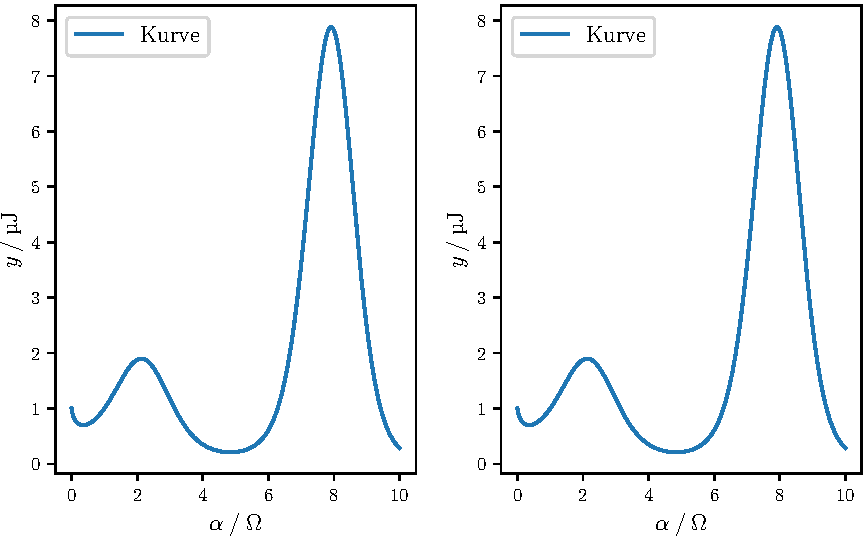
\includegraphics{plot.pdf}
%  \caption{Plot.}
%  \label{fig:plot}
%\end{figure}
